%%%%%%%%%%%%%%%%%%%%%%%%%%%%%%%%%%%%%%%%%%%%%%%%%%%%%%%%%%%%%%%%%%%%%%%%%%%%%%%%
% reconstruction.tex:
%%%%%%%%%%%%%%%%%%%%%%%%%%%%%%%%%%%%%%%%%%%%%%%%%%%%%%%%%%%%%%%%%%%%%%%%%%%%%%%%
\chapter{Event Reconstruction}
\label{sec:reco_chapter}
%%%%%%%%%%%%%%%%%%%%%%%%%%%%%%%%%%%%%%%%%%%%%%%%%%%%%%%%%%%%%%%%%%%%%%%%%%%%%%%%

Electrons, muons and jets expected from \WR and \nul decays were reconstructed from charged particle 
tracks measured by the silicon tracker, and energy deposits measured by the calorimeters and muon 
detectors.  The high expected energy of final state leptons and jets motivated the use of specific 
lepton and jet reconstruction algorithms described herein.  In general, these algorithms reconstructed 
charged particles by matching calorimeter energy clusters to reconstructed tracks, and reconstructed 
neutral particles from calorimeter energy clusters that did not match any reconstructed tracks.  
Representative trajectories of electrons, muons, and hadrons are shown in Figure \ref{fig:particleTrajectories}.

\begin{figure}[h]
	\centering
	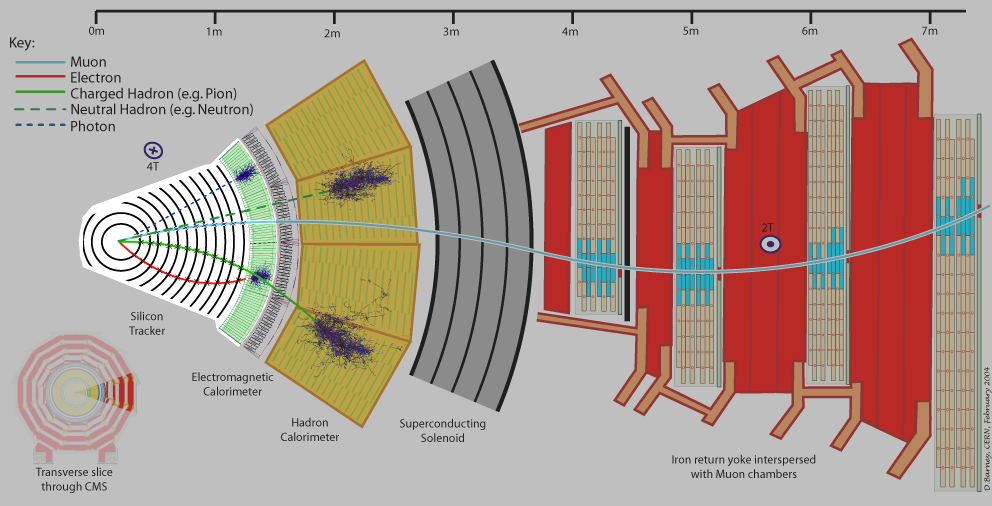
\includegraphics[width=1.0\textwidth]{figures/flowOfParticlesThroughCMS.gif}
	\caption{A typical trajectory of a muon and other particles travelling through CMS, from $European Laboratory for Particle Physics$.}
	\label{fig:particleTrajectories}
\end{figure}


\section{Electron Reconstruction}
\label{sec:eleReco}
Electrons ($\equiv e^{\pm}$) were the only particles considered in the \WR search that, on average, lost non-negligible 
amounts of energy in the tracker.  They lost energy through bremstrahhlung, and the resulting bremsstrahlung 
photons were detected outside the tracker by the ECAL.  Electron tracks were reconstructed from hits in 
individual tracker layers along helical paths using a dedicated algorithm that also estimated the energy lost.  
Reconstructed tracks determined electron $(\eta, \phi)$ trajectories, but ECAL measurements dictated their 
energies.

After traversing the tracker, electrons impinged on ECAL crystals and lost substantially all of their 
energy through radiative processes.  These processes resulted in showers of lower energy particles 
that enabled measurements of initial electron energies.  Showers of individual electrons in ECAL were usually 
3 or fewer crystals wide in $\eta$ and $\phi$, but electrons were reconstructed in 5 $\times$ 5 crystal 
superclusters (SCs) to recover bremsstrahlung photons, as shown in Figure \ref{fig:eleTrackAndSC}.  Following 
SC reconstruction, the $(\eta, \phi)$ positions of SCs were compared to 
the $(\eta, \phi)$ trajectories of electron candidate tracks.  Each reconstructed electron was identified 
as a SC and at least one track with matching $(\eta, \phi)$ coordinates.

\begin{figure}[h]
	\centering
	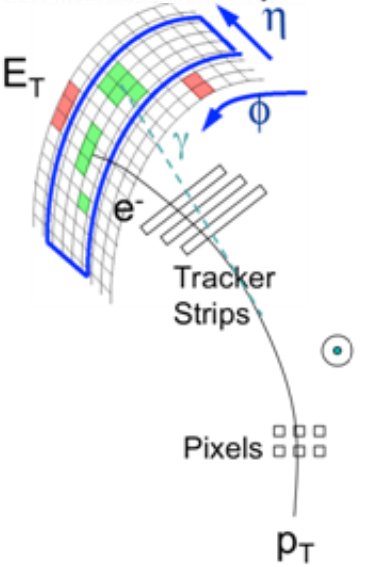
\includegraphics[width=1.0\textwidth]{figures/electronTrackAndSupercluster.png}
	\caption{An electron's trajectory through the tracker and ECAL.}
	\label{fig:eleTrackAndSC}
\end{figure}


\section{Muon Reconstruction}
\label{sec:muReco}
Muon ($\equiv \mu^{\pm}$) reconstruction started with reconstructing tracks in the silicon tracker.  
Hits in individual tracker layers were reconstructed into helical tracks, whose $(\eta, \phi)$ 
trajectories determined the directions of reconstructed muons.  Reconstructed tracks also provided 
initial muon momentum estimates that were further refined by muon detector measurements.

Muons, on average, lost negligible amounts of energy before entering the muon detectors.  Hits in 
muon chambers were reconstructed into helical tracks, and measuring their radii of curvature improved 
muon momentum resolution.  Muon detector tracks were extrapolated back to the silicon tracker, and 
then the $\eta$ and $\phi$ of silicon tracker and muon detector tracks were compared.  Each 
reconstructed muon was identified as a muon detector track whose trajectory matched a silicon 
tracker track.

The momentum of muons was determined using silicon tracker and muon detector measurements.  Four 
reconstruction algorithms fitted four continuous tracks \cite{cmsMuonRecoRunTwo} to silicon tracker and muon detector hits 
to estimate the muon's trajectory through all of CMS, represented in Figure \ref{fig:particleTrajectories}.  Each algorithm combined 
muon detector and silicon tracker measurements in a different way, and could exclude measurements 
with large uncertainty.  The precision of each continuous track was 
identified by a fit uncertainty $\chi^{2}/nDOF$ and momentum uncertainty $\sigma(\pt)/\pt$.  The 
track with the lowest fit and momentum uncertainties determined the reconstructed muon momenta.  
This procedure improved the momentum resolution for muons with $\pt > 200$ $\GeV$, which were 
expected in a significant fraction of $\WR \rightarrow \mu\mu jj$ events, as shown in Table 
\ref{tab:wrHighPtMuons}.

\begin{table}[h]
	\caption{Fraction of expected $\WR \rightarrow \mu\mu jj$ events that had at least one muon with $\pt > 200$ $\GeV$. 
	($\mnul = \frac{1}{2}\mWR$)}
	\label{tab:wrHighPtMuons}
	\centering
	\begin{tabular}{c|c}
		\mWR ($\TeV$) & Fraction of events with at least one high-$\pt$ muon (\%) \\  \hline
		1.0 &  80.  \\
		2.0 &  95.  \\ 
		3.0 &  98.  \\ \hline
	\end{tabular}
\end{table}


\section{Jet Reconstruction}
\label{sec:jetReco}
Through hadronization, photon radiation and leptonic weak decays, quarks produced in pp interactions 
created jets of photons, hadrons and leptons.  Jet reconstruction began by reconstructing photons, 
electrons and muons, and generic charged and neutral hadrons.  Each charged hadron was reconstructed as 
an energy measured in an HCAL tower geometrically matched to a reconstructed track.  In addition, 
charged hadrons could also contain an ECAL SC if the SC $(\eta, \phi)$ position was consistent with 
the HCAL tower.  Each neutral hadron was reconstructed as an HCAL tower, possibly associated with 
an ECAL SC, whose $(\eta, \phi)$ position was not consistent with any reconstructed track.  Similarly, 
each photon was reconstructed as an ECAL SC whose position was not consistent with any reconstructed 
track.  Subsequently, jets were reconstructed by clustering individual reconstructed particles together, 
as shown in Figure \ref{fig:jetClustering}.

\begin{figure}[h]
	\centering
	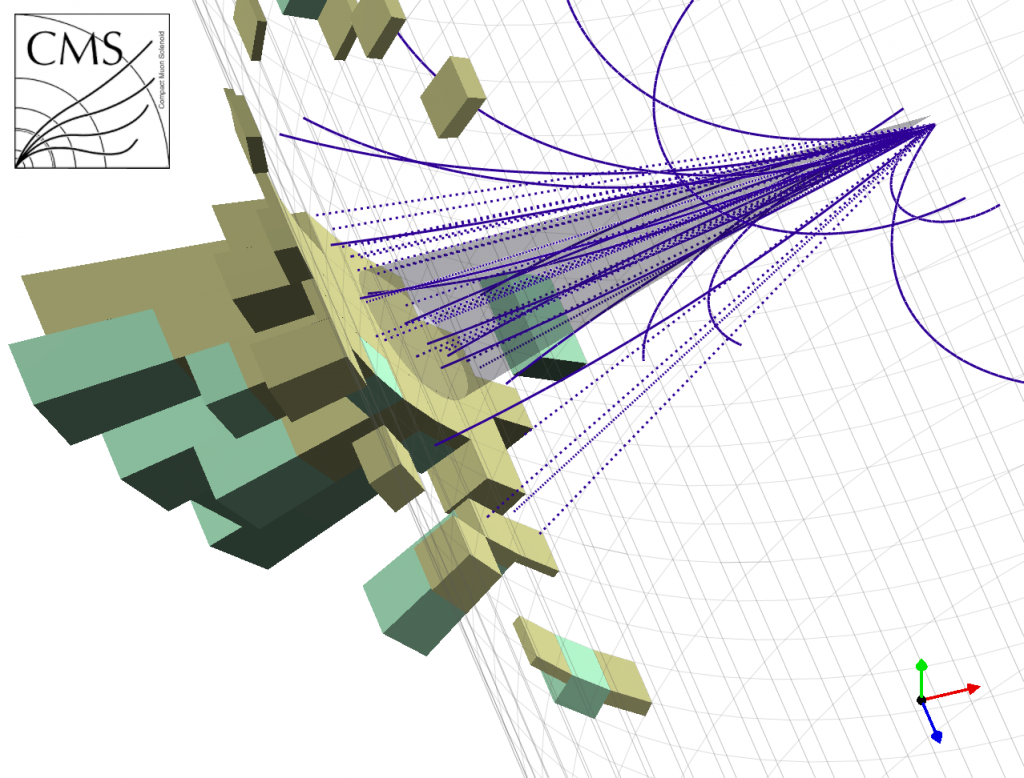
\includegraphics[width=1.0\textwidth]{figures/jetClusteringInCMS.png}
	\caption{A cone of reconstructed particles clustered into a jet, with the reconstructed vertex on the right.  
	From $CMS Experiment$.}
	\label{fig:jetClustering}
\end{figure}

In each event, every reconstructed particle was considered a jet candidate, except charged 
hadrons that did not originate from the reconstructed vertex with the highest $\sum \pt$.  Using the 
anti-$k_{T}$ algorithm \cite{antikt}, reconstructed particles were clustered into multi-particle jets 
based on their individual energies and trajectories.  Jet energies were equal to the total energy of 
all constituents, jet $(\eta, \phi)$ trajectories were defined as the energy-weighted average trajectory 
of all constituents, and the majority of each jet's energy was contained in a circular area with radius 
$\Delta R = 0.4$.


\section{Conclusion}
\label{sec:recoConclusion}
Energetic electrons, muons and jets produced by all types of interactions in pp collisions were 
reconstructed using several CMS subdetector systems.  Additional selections were applied to charged leptons 
and jets to isolate events with signs of a \WR and \nul.

%%%%%%%%%%%%%%%%%%%%%%%%%%%%%%%%%%%%%%%%%%%%%%%%%%%%%%%%%%%%%%%%%%%%%%%%%%%%%%%%
